\subsection{The latent variable motivation}

\begin{frame}{The latent variable motivation}
  \begin{itemize}
    \item<1-> Consider binary responses $y_1, \dots, y_n$ together with their corresponding covariates $x_1, \dots, x_n$. 
    \item<1-> For $i=1,\dots,n$, model the responses as
    \[
      y_i \sim \Bern(p_i).
    \]
    \item<2-> Assume that there exists continuous, underlying latent variables $y_1^*, \dots, y_n^*$, such that
    \[
      y_i =
      \begin{cases}
        1 & \text{ if } y_i^* \geq 0 \\
        0 & \text{ if } y_i^* < 0.    \\
      \end{cases}
    \]
    \item<3-> Model these continuous latent variables according to
    \[
      y_i^* = f(x_i) + \epsilon_i
    \]
    where $(\epsilon_1, \dots, \epsilon_n) \sim \N(\bzero, \bPsi^{-1})$ and $f \in \cF$ (some RKHS).
  \end{itemize}
\end{frame}

\subsection{Using I-priors}
\begin{frame}{Using I-priors}
  \vspace{-5pt}
  \begin{itemize}\setlength\itemsep{0.5em}
    \only<1|handout:0>{
    \item Assume an I-prior on $f$. Then,
    \begin{align*}
      \begin{gathered}
        f(x_i) = {\color{white} \overbrace{\color{black} f_0(x_i)}^{\alpha}} 
        + \sum_{k=1}^n h_\lambda(x_i, x_k)w_k \\
        (w_1, \dots, w_n) \sim \N(\bzero, \bPsi) \\
      \end{gathered}
    \end{align*}
    }
    \only<2->{
    \item Assume an I-prior on $f$. Then,
    \begin{align*}
      \begin{gathered}
        f(x_i) = {\color{gray} \overbrace{\color{black} f_0(x_i)}^{\alpha}} 
        + \sum_{k=1}^n h_\lambda(x_i, x_k)w_k \\
        (w_1, \dots, w_n) \sim \N(\bzero, \bPsi) \\
      \end{gathered}
    \end{align*}
    }
    \item<2-> For now, consider iid errors $\bPsi = \psi\bI_n$. \onslide<3->{In this case,
    \begin{align*}
      p_i = \Prob[y_i = 1] &= \Prob[y_i^* \geq 0] \\
      &= \Prob[\epsilon_i \leq f(x_i)] \\
      &= \Phi\Big(\psi^{1/2} ( 
%      {\color{gray} 
%      \underbrace{{\color{black} \alpha + {\textstyle\sum_{k=1}^n} h_\lambda(x_i, x_k)w_k}}_{\eta_i}
%      }
      \alpha + {\textstyle\sum_{k=1}^n} h_\lambda(x_i, x_k)w_k
      ) \Big)
    \end{align*}
    where $\Phi$ is the CDF of a standard normal.}
    \item<4-> No loss of generality compared with using an arbitrary threshold $\tau$ or error precision $\psi$. Thus, set $\psi = 1$.
  \end{itemize}
\end{frame}

\begin{frame}{The I-prior probit model}
  \begin{tikzpicture}[scale=1.1, transform shape]
    \tikzstyle{main}=[circle, minimum size = 10mm, thick, draw =black!80, node distance = 16mm]
    \tikzstyle{connect}=[-latex, thick]
    \tikzstyle{box}=[rectangle, draw=black!100]
      \node[main, draw=none] (fake) {};
      \node[main, fill = black!10] (H) [right=of fake, xshift=-1.65cm] {$x_i$};
      \node[main, double, double distance=0.6mm] (eta) [right=of H] {$f_i$};
      \node[main, double, double distance=0.6mm] (ystar) [right=of eta] {$p_i$};
      \node[main, draw=colblu] (lambda) [above=of H, xshift=0.4cm, yshift=-0.4cm] {\color{colblu} $\lambda$};  %
      \node[main, draw=colgre] (alpha) [above=of eta, yshift=0.3cm] {\color{colgre} $\alpha$};  
      \node[main, fill = black!10] (y) [right=of ystar] {$y_i$};
      \node[main, draw=colred] (w) [below=of eta, yshift=0.4cm] {\color{colred} $w_i$};  
      \path (alpha) edge [connect] (eta)
            (lambda) edge [connect] (eta)
    		(H) edge [connect] (eta) 
    		(eta) edge [connect] node [above] {$\Phi$} (ystar)
    		(ystar) edge [connect] (y)
    		(w) edge [connect] (eta)
            (H) edge [] node [above] {$h$} (eta);
      \node[rectangle, draw=black!100, fit= (H) (y) (w) ] {}; 
      \node[rectangle, fit= (w) (y), label=below right:{$i=1,\dots,n$}, xshift=-0.35cm, yshift=0.55cm] {};  % the label
    \end{tikzpicture}
    
    \begin{textblock*}{0.48\textwidth}(0.52\textwidth,0.55cm)
    \begin{block}{}
    \vspace{-1.6em}
      \begin{align*}
        &p(\by,\bw,\alpha,\lambda)  \\
        &= p(\by|\bff)p(\bw)p(\lambda)p(\alpha) \\
        &= {\textstyle\prod_{i=1}^n} \Phi(f_i)^{y_i} \big(1 - \Phi(f_i)\big)^{1-y_i} \\
        &\phantom{==} \cdot {\color{colred} [\N(0,1)]^n} 
        \cdot {\color{colblu} \N(\lambda_0,\kappa_0^{-1})} \\
        &\phantom{==} \cdot {\color{colgre} \N(\alpha_0,\tau_0^{-1})}
      \end{align*}
    \end{block}
  \end{textblock*}
\end{frame}

\subsection{Estimation (and challenges)}

\begin{frame}{Estimation}
  \vspace{5pt}
  \begin{columns}
    \uncover<1->{
    \begin{column}{0.47\textwidth}
      \vspace{6pt}
      \begin{itemize}\setlength\itemsep{0.5em}
        \item Denote $f_i = f(x_i)$ for short.
        \item The marginal density
        \vspace{4pt}
        \[
          \hspace{0.75cm} p(\by) = \int p(\by | \bff) p(\bff) \d\bff 
        \]
      \end{itemize}
    \end{column}}
    \uncover<4->{
    \begin{column}{0.5\textwidth}
    \vspace{-42pt}
      \begin{center}
        
\includegraphics[scale=0.40]{figure/taylor_expand_meme}
      \end{center}
    \end{column}}
  \end{columns}
  \uncover<1->{
  \vspace{-5pt}
  \[
    \phantom{p(\by)} = \int \prod_{i=1}^n \left[ \Phi(f_i)^{y_i} \big(1 - \Phi(f_i)\big)^{1-y_i} \right] \cdot \N(\alpha\bone_n, \bH_\lambda^2) \d\bff
  \]
  \hspace{0.65cm} for which $p(\bff|\by)$ depends, cannot be evaluated analytically.}
  \vspace{3pt}
  \begin{itemize}
    \item<2-> Some strategies:
    \begin{itemize}
      \item[\xmark]<2-> Naive Monte-Carlo integral
      \item[\xmark]<3-> EM algorithm with a MCMC E-step
      \item[{\color{FUorange}\cmark}]<4-> Laplace approximation
      \item[{\color{FUorange}\cmark}]<5-> MCMC sampling
    \end{itemize}
  \end{itemize}
\end{frame}

%\begin{frame}
%  \begin{center}
%    
\includegraphics[scale=0.5]{figure/taylor_expand_meme}
%  \end{center}
%\end{frame}

\begin{frame}{Laplace's method}
  \blfootnote{\fullcite[§4.1, pp. 777-778.]{Kass1995}}
  \vspace{-15pt}
  \begin{itemize}[<+->]\setlength\itemsep{0.8em}
    \item Interested in $p(\bff|\by) \propto p(\by|\bff)p(\bff) =: e^{Q(\bff)}$, with normalising constant $p(\by) = \int e^{Q(\bff)} \d\bff$. The Taylor expansion of $Q$ about its mode $\tilde\bff$
    \[
      Q(\bff) \approx Q(\tilde\bff) - \half (\bff - \tilde\bff)^\top\bA(\bff - \tilde\bff) 
    \]
    is recognised as the logarithm of an unnormalised Gaussian density, with $\bA = -\text{D}^2 Q(\bff)$ being the negative Hessian of $Q$ evaluated at  $\tilde\bff$.
    \item The posterior $p(\bff|\by)$ is approximated by $\N(\tilde\bff, \bA^{-1})$, and the marginal by
    \[
      p(\by) \approx (2\pi)^{n/2} \vert \bA \vert^{-1/2}  p(\by|\tilde\bff)p(\tilde\bff)
    \]
    \item Won't scale with large $n$; difficult to find modes in high dimensions.
  \end{itemize}
\end{frame}

\begin{frame}{Full Bayesian analysis using MCMC}
  \vspace{-3pt}
  \begin{itemize}\setlength\itemsep{0.5em}
    \item Assign hyperpriors on parameters of the I-prior, e.g.
    \begin{itemize}
      \item $\lambda^2 \sim \Gamma^{-1}(a,b)$
      \item $\alpha \sim \N(c,d^2)$
    \end{itemize}
    for a hierarchical model to be estimated fully Bayes.
    \item No closed-form posteriors - need to resort to MCMC sampling.
    \item Computationally slow, and sampling difficulty results in unreliable posterior samples.
  \end{itemize}
  \begin{center}
    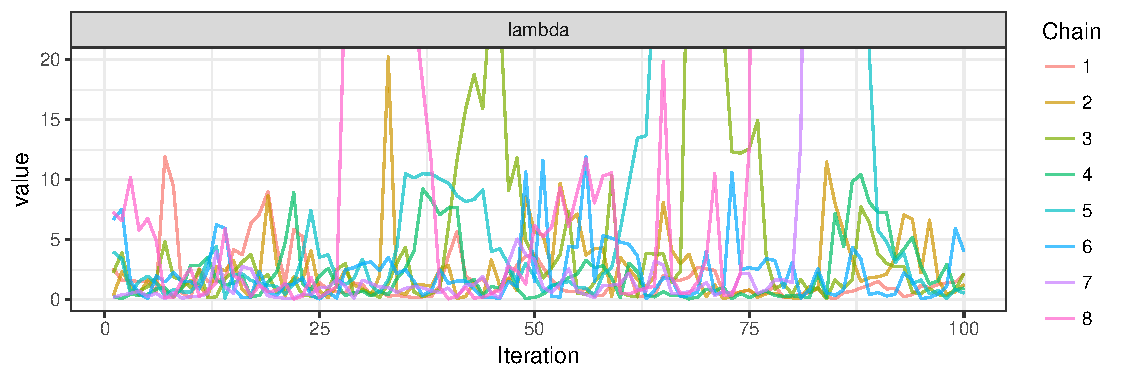
\includegraphics[scale=0.6]{mcmc1}
  \end{center}
\end{frame}








